\documentclass[fleqn,a4paper,12pt]{article}
\usepackage[german]{babel}
\usepackage[utf8]{inputenc} %Für Umlaute

\usepackage{amsmath}		% Mathematische Symbole
\usepackage{amssymb}		% Nochmehr mathematische Symbole
\usepackage{stmaryrd}		% Für die [[ ]] Klammern (\llbracket, \rrbracket)
\usepackage{dsfont}			% Schriftsatz fuer Zahlenmengensymbole
%\usepackage{verbatim}		% erweiterte Verbatim-Umgebung
\usepackage{alltt}			% Quasi-Verbatim-Umgebung
\usepackage{fancyhdr}		% Eigene Kopfzeilen
\usepackage{graphics}		% Zum Einbinden von Grafiken
\usepackage{tikz}			% Zur Erstellung von Graphen
% Einbinden einer eps-Grafik geht so: includegraphics{path}

% Seitenraender
\addtolength{\voffset}{-2cm}
\addtolength{\textheight}{0cm}
\addtolength{\hoffset}{0cm}
\addtolength{\textwidth}{2cm}
%\addtolength{\headheight}{2cm} % fuer jeden Strichkode einen Zentimeter

% Skalierung der Grafiken
\setlength{\unitlength}{1cm}

\pagestyle{fancy}				% Eigene Kopfzeilen verwenden
\frenchspacing					% Kein Extrafreiraum nach Satzzeichen
\setlength{\parindent}{0pt}		% Neue Absaetze nicht einruecken
%\sloppy						% Schlampige Absatzformatierung
\fussy							% Penible Absatzformatierung
\linespread{1.5}				% Zeilenabstand

%tikz-definition
\tikzstyle{rec} = [minimum width=1cm, minimum height=0.8cm, align = left,text centered, draw=black]

%andere Definitionen
\newcommand{\R}{{\mathbb R}}
\newcommand{\N}{{\mathbb N}}
\newcommand{\Z}{{\mathbb Z}}
\newcommand{\Q}{{\mathbb Q}}
\newcommand{\C}{{\mathbb C}} 
\newcommand{\F}{\mathcal{F}}
\newcommand{\less}{\setminus}
\newcommand{\inv}{{}^{-1}}
\newcommand{\Land}{\bigwedge}
\newcommand{\Lor}{\bigvee}

\begin{document}
	\begin{tabular}{l l}
		Funktion:		& $f(x) = -x \cdot \text{ld}(x) = -x\cdot{\log(x)}{\log(2)},\ x\in(0,1]$\\
		Domain:			& $\left\lbrace x\in\R\mid 0 < x \le 1\right\rbrace$\\
		Image:			& $\left\lbrace f(x)\in\R\mid 0 \le f(x) \le f\left(\frac{1}{e}\right) \right\rbrace$\\
		Graph:			& 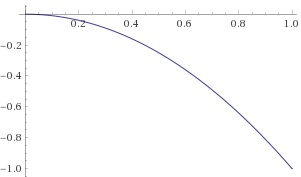
\includegraphics{plot-x2.jpg}\\
		1. Ableitung:	& $\frac{d}{dx}f(x) = $\\
		2. Ableitung:	& $\frac{d^2}{dx^2}f(x) = $\\
		3. Ableitung:	& $\frac{d^3}{dx^3}f(x) = $\\
		Stammfunktion:	& $F(x) = $???\\
						& $\int_0^1 f(x) dx = $\\
		Supremum:		& $f\left(\frac{1}{e}\right)$\\
		Maximum:		& $f\left(\frac{1}{e}\right)$\\
		Infimum:		& $0$\\
		Minimum:		& $f(1) = 0$\\
		Nullstellen:	& $x_0 = 1$\\
		Wendepunkt:		& -\\
		Scheitelpunkt:	& -\\
		Monotonie:		& $x\in\left(0,\frac{1}{e}\right)$ streng monoton wachsend\\
						& $x\in\left(\frac{1}{e},1\right]$ streng monoton fallend
						
	\end{tabular}
\end{document}